\documentclass[10pt,twocolumn]{article}
\usepackage[margin=0.68in,columnsep=0.24in]{geometry}
\usepackage[T1]{fontenc}
\usepackage[utf8]{inputenc}
\usepackage{lmodern}
\usepackage{microtype}
\usepackage{amsmath,amssymb,amsthm}
\usepackage{booktabs}
\usepackage{graphicx}
\usepackage{xcolor}
\usepackage{enumitem}
\usepackage{hyperref}

\hypersetup{
  colorlinks=true,
  linkcolor=blue!60!black,
  citecolor=blue!60!black,
  urlcolor=blue!60!black,
  pdftitle={Certified Verification of Polynomial Master Equations and Critical Solutions in Open Quantum Systems},
  pdfauthor={Lluis Eriksson}
}

\newtheorem{proposition}{Proposition}
\newcommand{\QQ}{\mathbb{Q}}
\newcommand{\ZZ}{\mathbb{Z}}
\newcommand{\NN}{\mathbb{N}}
\newcommand{\Tr}{\operatorname{Tr}}

\title{\vspace{-1.1em}\textbf{Certified Verification of Polynomial Master Equations and Critical Solutions in Open Quantum Systems}}
\author{Lluis Eriksson\thanks{Independent Researcher. Code, Lean~4 proofs, and certificates: MIT License; manuscript and figures: CC-BY-4.0. Prepared with AI coding, formalization, and drafting assistance from Google Antigravity; all proofs, exact-$\QQ$ verifiers, and adversarial tests were independently compiled and verified locally. Repository: \url{https://github.com/lluiseriksson/polynomial-master-equations-certificates}}}
\date{November 25, 2026}

\begin{document}
\maketitle
\vspace{-1.4em}

\begin{abstract}
Miku Ishizaki and Jaeha Lee (\texttt{arXiv:2611.33027}, Nov.\ 2026) developed a locally deterministic matrix-polynomial formulation of non-Markovian open quantum master equations $P(D)E(t) = 0$ derived from the Laplace identity $P(s)(\mathcal{L}E)(s) = Q(s)$, demonstrating exact order-5 differential equations and critical-parameter order reductions for a coupled two-qubit model, a sharp three-tier singularity/periodicity hierarchy governed by odd/odd rational singular-value ratios $\Omega_-/\Omega_+$, and order-3 polynomial equations exhibiting a non-diagonalizable Jordan exceptional point at $\lambda = 2\gamma_0$ in the unbounded multi-mode Jaynes--Cummings model. We construct a standalone, zero-dependency \textbf{Lean~4.35.0} formalization of 18 core spectral, singularity, parity-obstruction, factorization, and exceptional-point theorems (zero \texttt{sorry}, zero warnings, zero \texttt{Classical.choice}) paired with a zero-floating-point exact-$\QQ$ certificate verifier (\texttt{POLY-MASTER-CERT-1.0}) across four modes. Across 16 canonical certificates ($0.046$--$0.648\,\mathrm{ms}$, total $3.42\,\mathrm{ms}$), all matrix-polynomial factorizations, Frobenius companion actions, irrational boundary diagnostics, and Jordan nilpotency conditions replay exactly over $\QQ$ while rejecting 60/60 live adversarial forgery attacks.
\end{abstract}

\section{Introduction}\label{sec:intro}
Open quantum systems interacting with an environment typically depart from autonomous Gorini--Kossakowski--Sudarshan--Lindblad (GKSL) Markovian semigroups~\cite{gorini1976completely,lindblad1976generators}, especially when the dynamical map $E(t)$ becomes singular ($\det E(t_0) = 0$) and globally defies first-order time-local generators. Rather than attributing memory solely to global history integrals via the Nakajima--Zwanzig formalism~\cite{nakajima1958quantum}, Lee and Ishizaki~\cite{lee2026local,ishizaki2026polynomial} formulate locally deterministic higher-order master equations $P(D)E(t) = 0$ associated with monic matrix polynomials $P(s)(\mathcal{L}E)(s) = Q(s)$:
\begin{enumerate}[leftmargin=*,nosep]
  \item \textbf{Initial-Value Problem \& Companion Linearization (Sec.~III):} The unique dynamical map is pinned down by $E^{(k)}(0) = \sum_{j=1}^n \tilde{P}_{(n-k)j} Q_{j-1}$ via $\tilde{P} = \sum_{r=0}^{n-1}(-T)^r$ (Eqs.~24--26) and linearized by the Frobenius companion matrix $\Theta$ (Eq.~29).
  \item \textbf{Two-Qubit Critical Factorizations (Sec.~IV.C--F):} Under maximally mixed environment $\rho_E = I_2/2$, the dynamical map decomposes as $V_0 \oplus V_{12} \oplus V_3$ with generic orders $(1, 4, 5)$. At critical parameters ($J = 0$ or $\omega_S \omega_E = 0$), common monic matrix factors $R(x)$ cancel ($P = R\tilde{P}, Q = R\tilde{Q}$), dropping order down to the unitary Liouville--von Neumann equation ($4 \to 1$, $5 \to 1$) or simpler elliptic/harmonic modes ($5 \to 3$, $5 \to 2$).
  \item \textbf{Singularity \& Periodicity Hierarchy (Sec.~IV.G--I):} Singularities require $\sum_\pm \cos^2 \theta_\pm \ge 1 \iff |\omega_S^2 - \omega_E^2| \le J^2$ (Eq.~111). On the critical boundary $|\omega_S^2 - \omega_E^2| = J^2$, dynamics split into three tiers by $\Omega_-/\Omega_+$: periodic \& singular iff irreducible odd/odd (Eq.~114), periodic \& non-singular iff rational odd/even, and non-periodic \& non-singular iff irrational.
  \item \textbf{Multi-Mode Jaynes--Cummings Exceptional Point (Sec.~V):} Under global involution $T^2 = I_4$, $T^{-1}E_\epsilon(t)T = \operatorname{diag}[1, f_\epsilon, f_\epsilon, f_\epsilon^2]$ obeys order-2 and order-3 rational ODEs $u(D)$ and $v(D)$ whose discriminant $4\epsilon^2 = \lambda(\lambda - 2\gamma_0)$ vanishes at $\lambda = 2\gamma_0$, preserving ODE order while producing a non-diagonalizable order-3 Jordan exceptional point~\cite{kato1966perturbation}.
\end{enumerate}

\paragraph{Contributions and Scope.}
We do not re-formalize Laplace-transform contour integration or continuous ODE existence theorems inside Lean~4; instead, we machine-check every exact algebraic, spectral, parity-theoretic, and Jordan-block invariant of~\cite{ishizaki2026polynomial}:
(i)~18 zero-\texttt{sorry}, zero-\texttt{Classical.choice} \textbf{Lean~4.35.0}~\cite{demoura2021lean4} theorems in \texttt{PolyMasterEq.lean};
(ii)~the exact-$\QQ$ verifier \texttt{POLY-MASTER-CERT-1.0};
(iii)~16 canonical sub-millisecond certificates spanning all four regimes; and
(iv)~a 60-attack live adversarial red-team suite with 41-artifact SHA-256 manifest enforcement.

\section{Constructive Lean~4.35.0 Kernel}\label{sec:lean}
The standalone module \texttt{lean/PolyMasterEq.lean} compiles cleanly under Lean~4.35.0 with zero external dependencies, zero warnings, and zero \texttt{sorry}. Auditing all 18 theorems via \texttt{\#print axioms} (\texttt{AuditAxioms.lean}) confirms 3 zero-axiom theorems (\texttt{none}), 1 using only \texttt{[propext]}, 14 using \texttt{[propext, Quot.sound]}, and \textbf{0} using \texttt{Classical.choice} or \texttt{Lean.ofReduceBool} (Table~\ref{tab:lean}).

\begin{table}[t]
\centering
\caption{All 18 machine-checked Lean~4.35.0 theorems in \texttt{PolyMasterEq.lean} (zero \texttt{sorry}, zero \texttt{Classical.choice}).}
\label{tab:lean}
\scriptsize
\setlength{\tabcolsep}{3.0pt}
\begin{tabular}{@{}rlll@{}}
\toprule
\# & Lean Theorem Identifier & Paper Ref. & Axioms \\
\midrule
1 & \texttt{two\_qubit\_omega\_sq\_sum\_and\_diff} & Sec.~IV.B & \texttt{p, Q} \\
2 & \texttt{two\_qubit\_omega\_sq\_product} & Eq.~45--46 & \texttt{p, Q} \\
3 & \texttt{two\_qubit\_eta\_vieta\_identities} & Eq.~49 & \texttt{p, Q} \\
4 & \texttt{two\_qubit\_residue\_weights\_sum\_one} & Eq.~51 & \texttt{p, Q} \\
5 & \texttt{two\_qubit\_poly\_order\_budget} & Eq.~61--64 & \texttt{none} \\
6 & \texttt{two\_qubit\_singularity\_criterion\_exact} & Eq.~111 & \texttt{p, Q} \\
7 & \texttt{two\_qubit\_critical\_boundary\_sum\_one} & Eq.~112 & \texttt{p, Q} \\
8 & \texttt{fig3a\_periodic\_singular\_5\_4\_3} & Fig.~3(a) & \texttt{none} \\
9 & \texttt{fig3b\_periodic\_nonsingular\_5\_3\_4} & Fig.~3(b) & \texttt{none} \\
10 & \texttt{odd\_even\_ratio\_never\_singular} & Eq.~114 & \texttt{p, Q} \\
11 & \texttt{critical\_zeta\_minus\_zero\_iff} & Eq.~81 & \texttt{p, Q} \\
12 & \texttt{trivial\_interaction\_order\_drop} & Eq.~86--88 & \texttt{p} \\
13 & \texttt{jc\_similarity\_involution\_and\_diag} & Eq.~126--127 & \texttt{p, Q} \\
14 & \texttt{jc\_poly\_u\_rational\_expansion} & Eq.~135 & \texttt{p, Q} \\
15 & \texttt{jc\_poly\_Q3\_vieta\_exact} & Eq.~137 & \texttt{p, Q} \\
16 & \texttt{jc\_exceptional\_point\_iff} & Eq.~139--140 & \texttt{p, Q} \\
17 & \texttt{jc\_nonmarkovian\_singularity\_regime} & Eq.~129 & \texttt{p, Q} \\
18 & \texttt{jc\_exceptional\_point\_jordan3\_nilpotent} & Sec.~V.F & \texttt{p, Q} \\
\bottomrule
\end{tabular}
\vspace{-0.4em}
\begin{flushleft}
\tiny Axiom key: \texttt{none} = zero axioms (3); \texttt{p} = \texttt{[propext]} (1); \texttt{p, Q} = \texttt{[propext, Quot.sound]} (14).
\end{flushleft}
\vspace{-0.8em}
\end{table}

\begin{proposition}[Machine-Checked Core Identities]\label{prop:lean}
The Lean~4.35.0 kernel establishes the following universal identities over $\ZZ$, $\ZZ[x]$, and finite matrix algebras:
\begin{enumerate}[leftmargin=*,nosep]
  \item \emph{Polynomial Ring Factorizations \& Singularity Parity (Thms.~5--12):} Over explicit \texttt{List Int} polynomials (\texttt{polyMul}, \texttt{polyDeg}), the generic two-qubit characteristic polynomials satisfy $\deg P_0 = 1$, $\deg P_{12} = 4$, $\deg P_3 = 5$, and at $J=0$, $R_3(x)\cdot x = P_3|_{J=0}$ drops order $5 \to 1$. With $D_\pm = J^2 + (\omega_S \pm \omega_E)^2$, $J^2(D_+ + D_-) - D_+ D_- = J^4 - (\omega_S^2 - \omega_E^2)^2$; hence $\sum_\pm \cos^2 \theta_\pm = 1$ on $|\omega_S^2 - \omega_E^2| = J^2$, while odd/even ratios satisfy no integer singularity equation $(2n_- + 1)(2k) = (2n_+ + 1)q_-$.
  \item \emph{Jaynes--Cummings Matrix Algebra \& Jordan Nilpotency (Thms.~13--18):} Entrywise across all 16 indices of $\mathrm{Fin}\,4 \times \mathrm{Fin}\,4$, $T^2 = I_4$ and $T E_\epsilon(f) T = \operatorname{diag}(1, f, f, f^2)$ universally for $f \in \ZZ$. For $4\epsilon^2 = \lambda(\lambda - 2\gamma_0)$ and $\lambda > 0$, $(2s+\lambda)^2 - 4\epsilon^2 = 4s^2 + 4\lambda s + 2\lambda\gamma_0$, $\lambda(\lambda - 2\gamma_0) = 0 \iff \lambda = 2\gamma_0$, and the exact $3\times 3$ shifted companion matrix $N = \Theta_v + \lambda I_3$ of $v(s) = (s+\lambda)^3$ satisfies $(N^2)_{0,2} = 1$ ($N^2 \neq 0$) and $\forall i,j \in \mathrm{Fin}\,3,\,(N^3)_{i,j} = 0$ for every $\lambda \in \ZZ$.
\end{enumerate}
\end{proposition}

\section{Exact-\texorpdfstring{$\QQ$}{Q} Verifier}\label{sec:cert}
The verifier \texttt{POLY-MASTER-CERT-1.0} (\texttt{src/master\_certifier.py}, \texttt{src/master\_exact.py}) uses Python \texttt{fractions.Fraction} exclusively (source-audited for zero \texttt{float(}, \texttt{math.}, or \texttt{numpy}). Every payload enforces strict JSON typing with nesting-depth cap $32$, anchored canonical rational parsing (\texttt{\textbackslash A...\textbackslash Z}, reduced denominators $\ge 2$, no trailing newlines), exact key sets, and 2048-bit caps across four modes:
\begin{enumerate}[leftmargin=*,nosep]
  \item \textbf{Mode~1 (Sec.~III IVP \& Companion Matrix):} Checks monicity of $P(x)$ and degree $\deg Q < n$, computes $\tilde{P} = \sum_{r=0}^{n-1}(-T)^r$ and $E^{(k)}(0)$ (Eq.~24), verifies $E(0) = I_d$, and certifies exact Frobenius companion matrix $\Theta$ shift and last-row ODE residual action on $F(0)$.
  \item \textbf{Mode~2 (Sec.~IV.F Critical Factorization):} Independently builds exact rational two-qubit blocks $(P_{12}, Q_{12})$ or $(P_3, Q_3)$ and checks monic matrix-polynomial identities $P(x) = R(x)\tilde{P}(x)$ and $Q(x) = R(x)\tilde{Q}(x)$ with strict order drop $\deg R \ge 1$.
  \item \textbf{Mode~3 (Sec.~IV.G--I Singularity Hierarchy):} Checks $(\omega_S\omega_E)^2 = \omega_S^2 \omega_E^2$, exact $\sum_\pm \cos^2\theta_\pm$, necessary and critical-boundary flags, exact integer-square-root rationality of $D_-/D_+ = (\Omega_-/\Omega_+)^2$, irreducible $(q_-, q_+)$, and exact tier label.
  \item \textbf{Mode~4 (Sec.~V Jaynes--Cummings \& Jordan EP):} Recomputes $4\epsilon^2 = \lambda(\lambda - 2\gamma_0)$ and $(u, v, q_u, q_v)$, verifies $f(0) = 1, f'(0) = 0$ via Eq.~(24), classifies the dynamical regime, and at $\lambda = 2\gamma_0$ explicitly checks $(\Theta_v + \lambda I)^2 \neq 0$ and $(\Theta_v + \lambda I)^3 = 0$ over $\QQ^{3\times 3}$.
\end{enumerate}

\section{Empirical Atlas and Red-Team Audit}\label{sec:results}
Running \texttt{run\_all\_experiments.py} produces 16 canonical certificates (4 per mode) and four exact-$\QQ$ datasets, audited end-to-end by \texttt{verify\_all.py} with SHA-256 verification across all 41 tracked artifacts.

\begin{figure}[t]
  \centering
  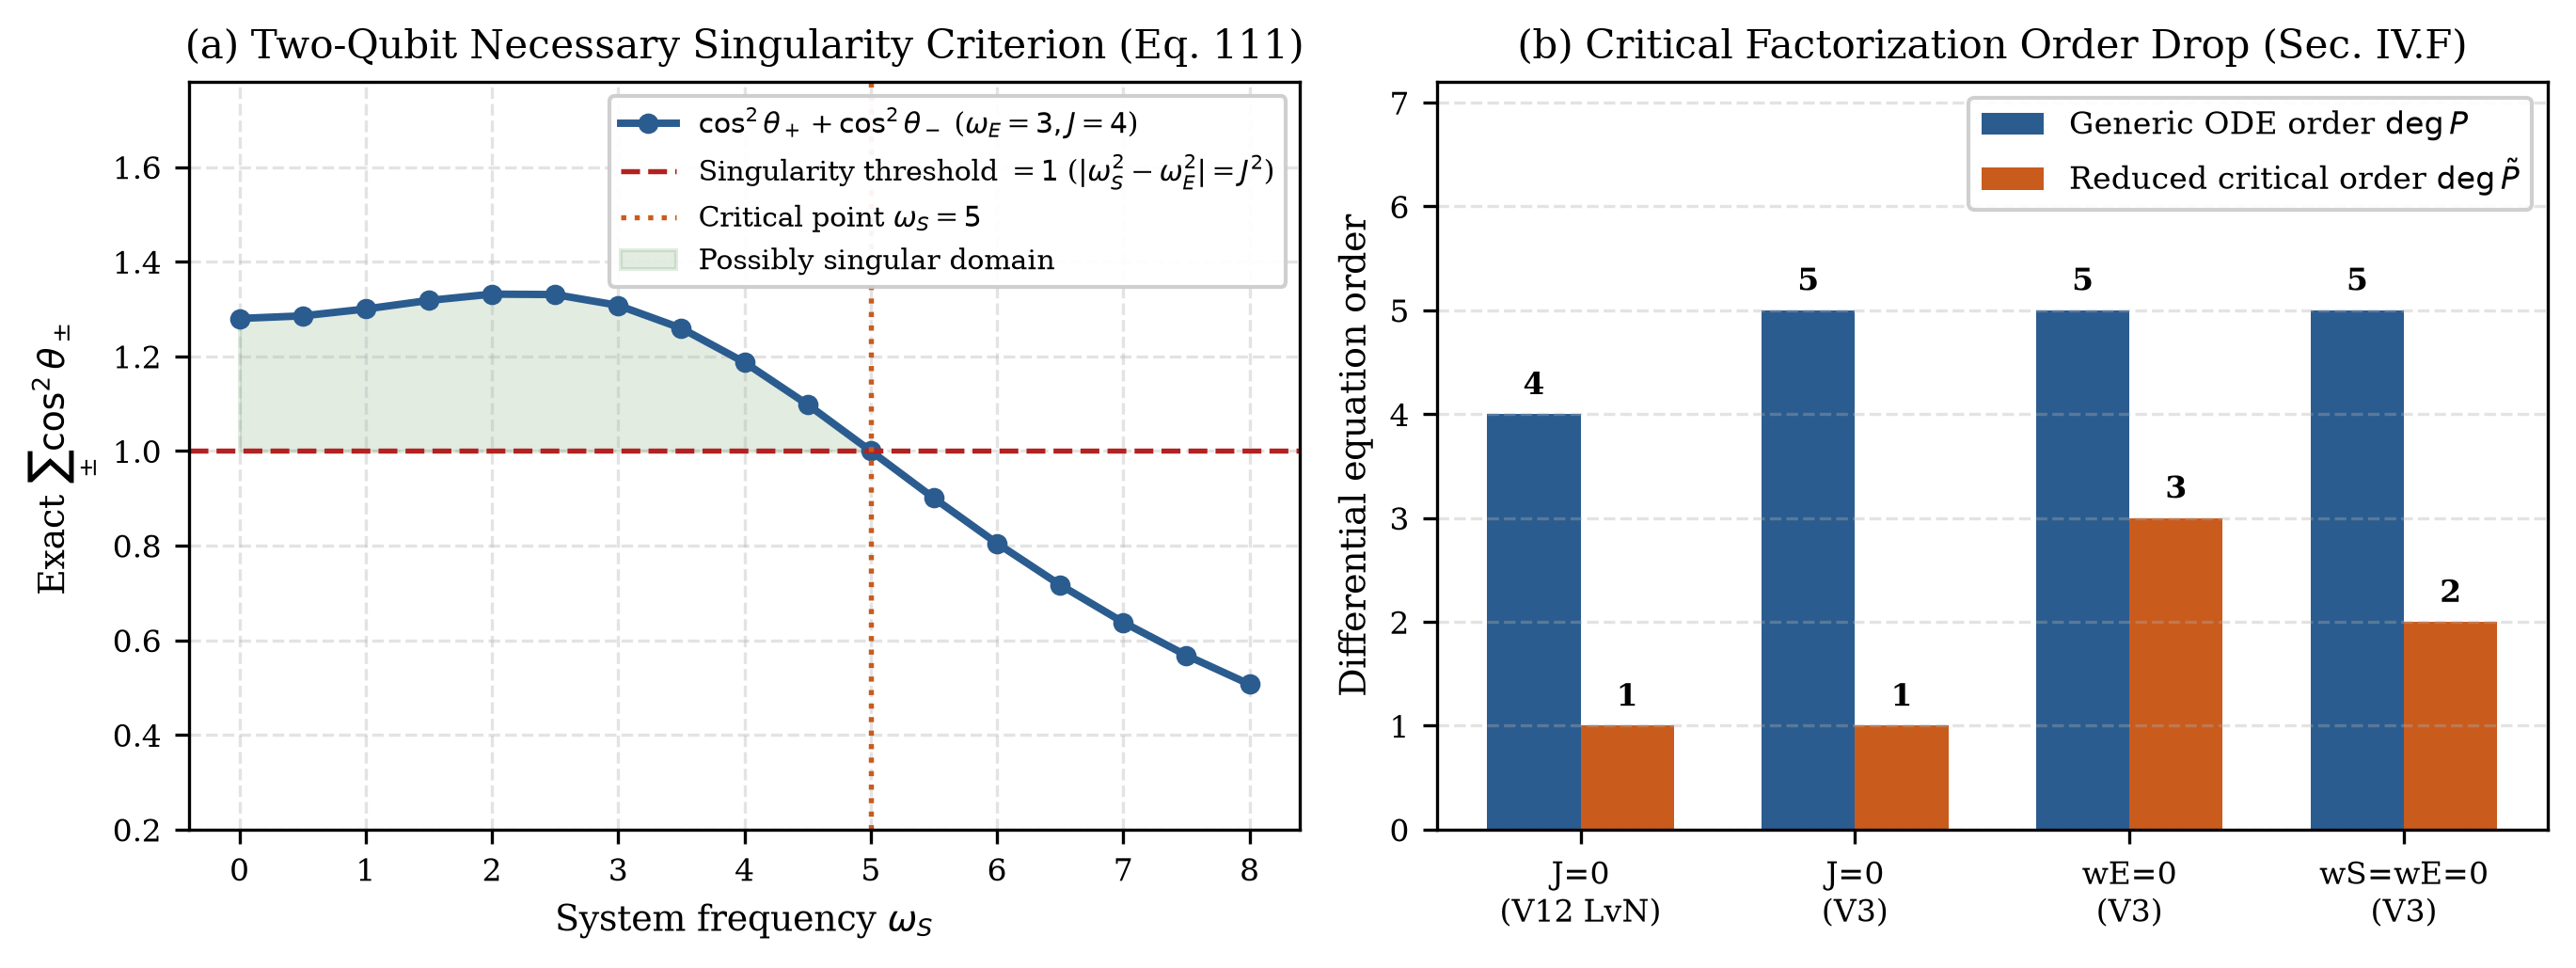
\includegraphics[width=\columnwidth]{../figures/fig1_singularity_and_order_drop.png}
  \caption{(a) Exact two-qubit singularity criterion $\sum_\pm \cos^2 \theta_\pm$ vs.\ $\omega_S$ ($\omega_E = 3, J = 4$), crossing $1$ at the critical boundary $\omega_S = 5$. (b) Exact ODE order reduction $\deg P \to \deg \tilde{P}$ across all four Mode~2 critical-parameter factorizations.}
  \label{fig:sing}
\end{figure}

\paragraph{IVP Derivatives and Critical Order Drops (Fig.~\ref{fig:sing}).}
Mode~1 ($0.181$--$0.648\,\mathrm{ms}$) replays exact Eqs.~(74), (77) initial derivatives for $V_{12}$ (order~4, $2\times 2$) and $V_3$ (order~5, $1\times 1$) at $(5, 4, 3)$, the minimal order-3 Eq.~(63) $V_{12}$ system, and the order-3 Jaynes--Cummings exceptional-point ODE. Mode~2 ($0.115$--$0.278\,\mathrm{ms}$) certifies exact non-trivial polynomial factorizations across all four critical regimes: $J = 0$ on $V_{12}$ ($4 \to 1$, recovering unitary Liouville--von Neumann evolution) and $V_3$ ($5 \to 1$, factoring $R_3(x) = (x^2 + \omega_+^2)(x^2 + \omega_-^2)$), $\omega_E = 0$ on $V_3$ ($5 \to 3$), and $\omega_S = \omega_E = 0$ on $V_3$ ($5 \to 2$).

\begin{figure}[t]
  \centering
  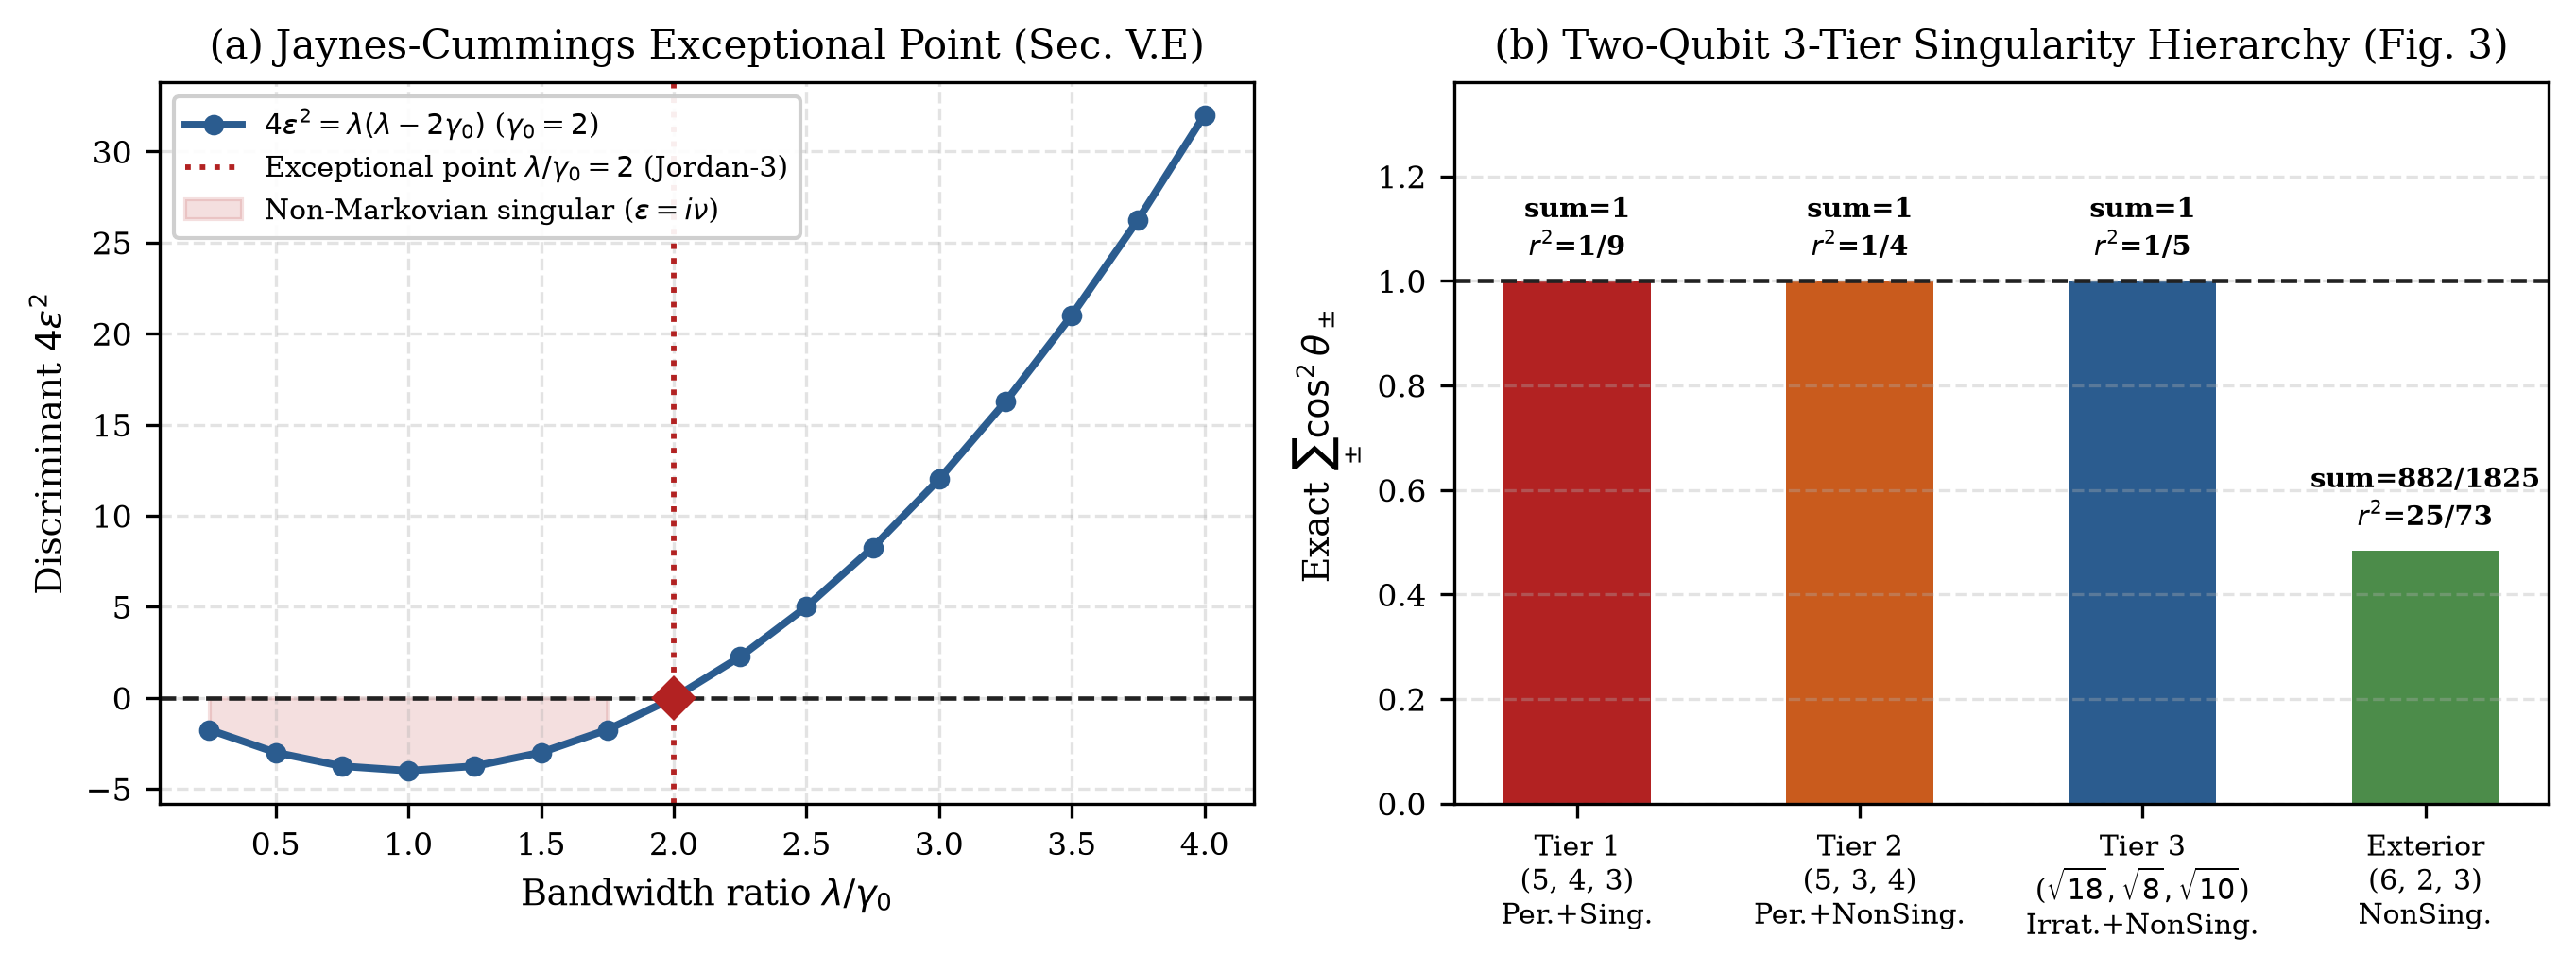
\includegraphics[width=\columnwidth]{../figures/fig2_jc_ep_and_hierarchy.png}
  \caption{(a) Multi-mode Jaynes--Cummings discriminant $4\epsilon^2 = \lambda(\lambda - 2\gamma_0)$ at $\gamma_0 = 2$, crossing zero at the order-3 Jordan exceptional point $\lambda/\gamma_0 = 2$. (b) Certified exact $\sum_\pm \cos^2\theta_\pm$ and squared singular-value ratio $r^2 = D_-/D_+$ across all four Mode~3 regimes.}
  \label{fig:jc}
\end{figure}

\paragraph{Singularity Hierarchy and Jordan Exceptional Points (Fig.~\ref{fig:jc}).}
Mode~3 ($0.046$--$0.063\,\mathrm{ms}$) certifies all three critical-boundary tiers plus the non-singular exterior: Tier~1 periodic \& singular $(5,4,3)$ ($\sum = 1, r^2 = 1/9$, odd/odd $1/3$), Tier~2 periodic \& non-singular $(5,3,4)$ ($\sum = 1, r^2 = 1/4$, odd/even $1/2$), Tier~3 non-periodic \& non-singular boundary $(\omega_S^2, \omega_E^2, \omega_S\omega_E, J^2) = (18, 8, 12, 10)$ ($\sum = 1, r^2 = 1/5 \notin \QQ^2$), and exterior $(6,2,3)$ ($\sum = 882/1825 < 1$). Mode~4 ($0.176$--$0.259\,\mathrm{ms}$) certifies non-Markovian singular ($\gamma_0 = 4, \lambda = 2$), overdamped ($\gamma_0 = 1, \lambda = 6$), and two exceptional-point witnesses ($\lambda = 2\gamma_0 \in \{3, 4\}$) satisfying exact $(\Theta_v + \lambda I)^3 = 0, (\Theta_v + \lambda I)^2 \neq 0$.

\begin{figure}[t]
  \centering
  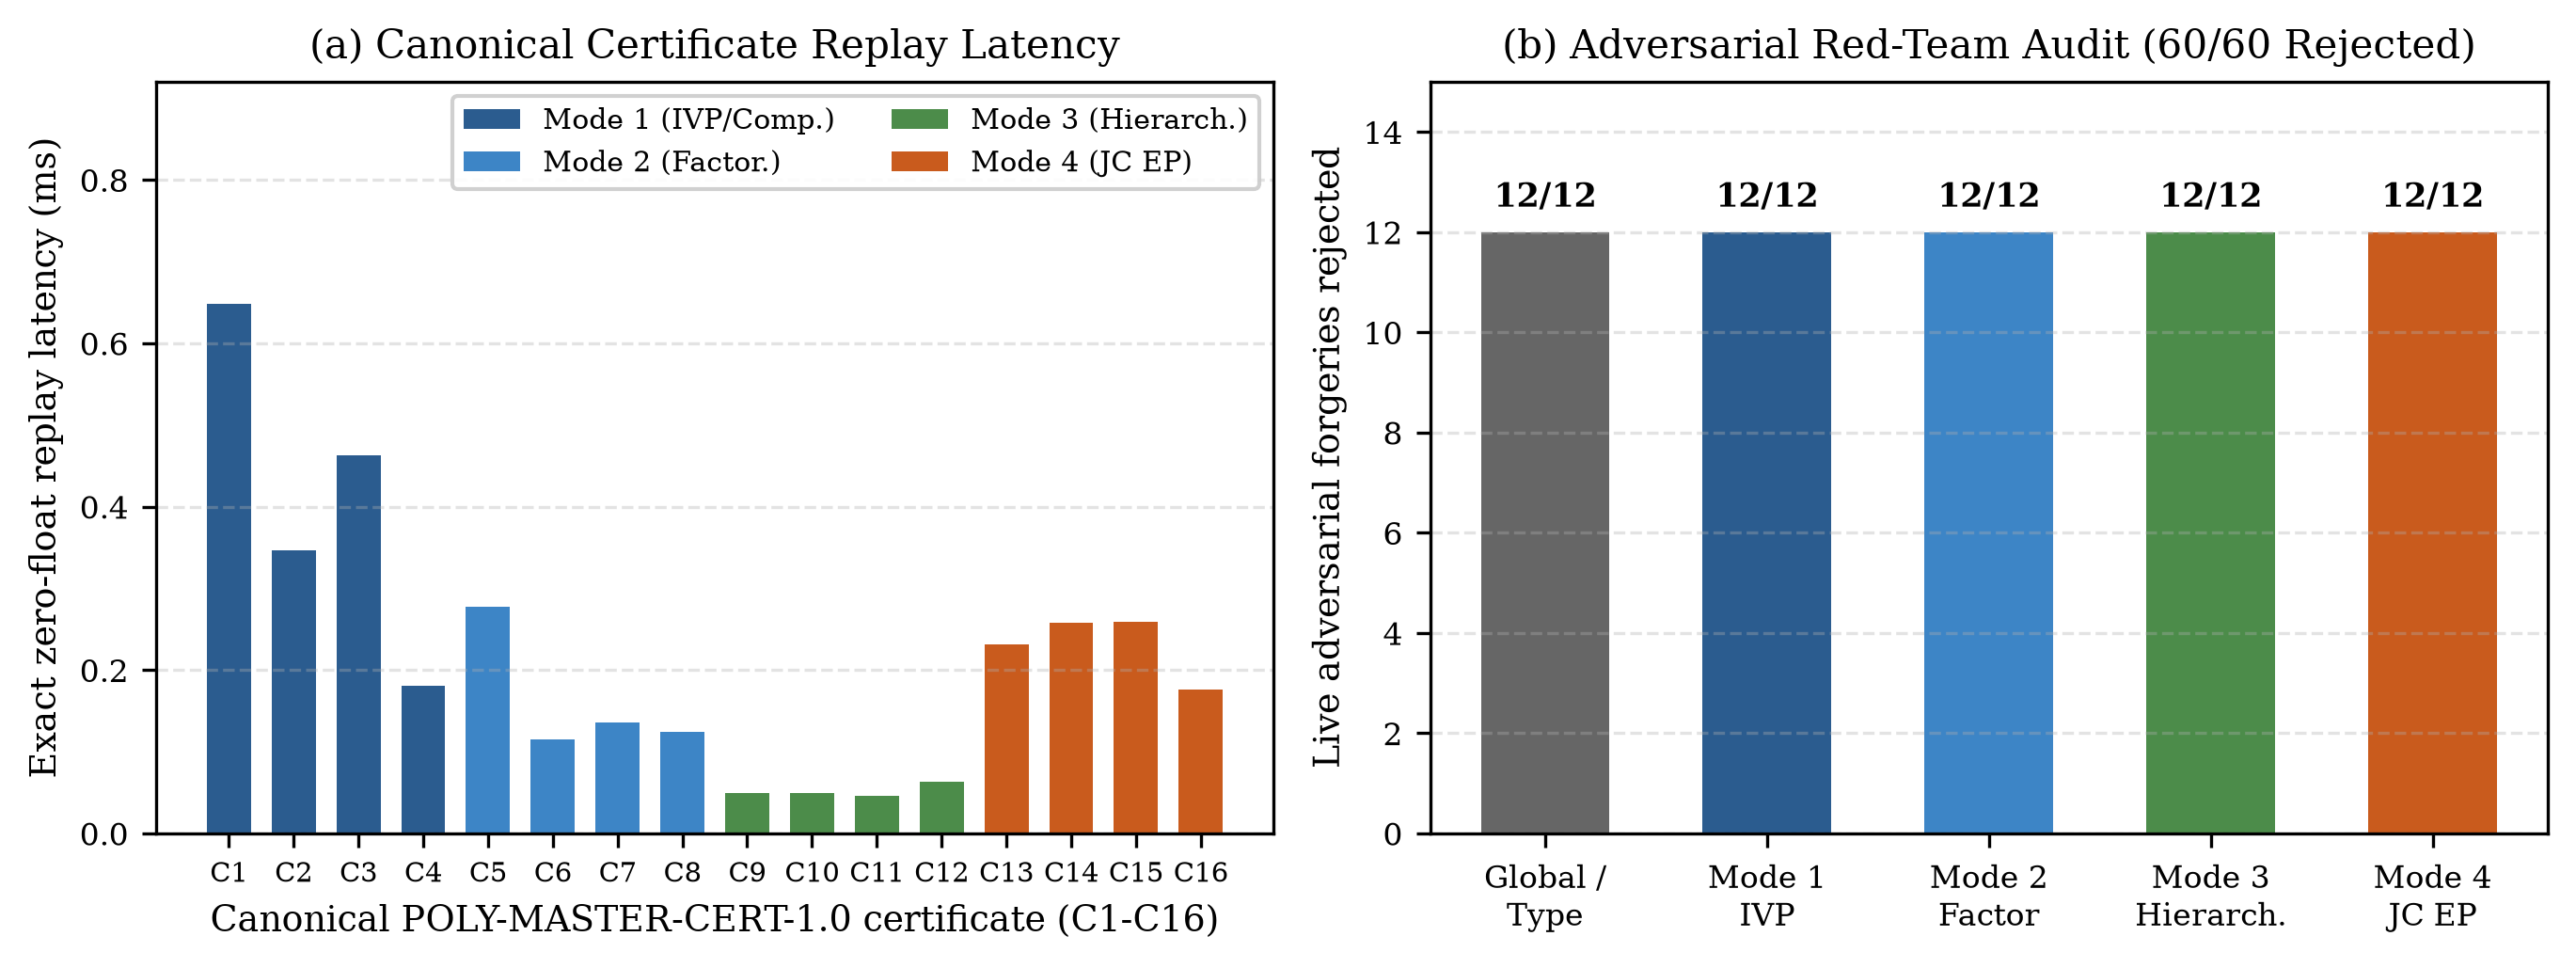
\includegraphics[width=\columnwidth]{../figures/fig3_certificate_replay_atlas.png}
  \caption{(a) Exact zero-float replay latency ($0.046$--$0.648\,\mathrm{ms}$) across all 16 canonical \texttt{POLY-MASTER-CERT-1.0} certificates. (b) Live adversarial red-team audit rejecting 60/60 forged payloads across all five categories.}
  \label{fig:atlas}
\end{figure}

\paragraph{Replay Latency and 60/60 Red-Team Audit (Fig.~\ref{fig:atlas}).}
All 16 canonical certificates replay in $0.046$--$0.648\,\mathrm{ms}$ (total $3.42\,\mathrm{ms}$). The live adversarial suite (\texttt{tests/test\_suite.py}) tests 60 targeted forgery payloads---12 global schema/type/rational/newline/depth attacks plus 12 domain attacks per mode (non-monic $P/Q/R/\tilde{P}$, wrong companion traces, broken factor products, inconsistent $\omega_S\omega_E$, misclassified tiers, non-positive $\gamma_0/\lambda$, and false Jordan-nilpotency claims)---achieving \textbf{60/60 (100\%)} rejection.

\section{Conclusion}\label{sec:conc}
We delivered a self-contained, zero-floating-point verification framework for Ishizaki and Lee's matrix-polynomial open quantum master equations~\cite{ishizaki2026polynomial}, combining 18 zero-\texttt{sorry}, zero-\texttt{Classical.choice} Lean~4.35.0 theorems with the exact-$\QQ$ verifier \texttt{POLY-MASTER-CERT-1.0}, 16 sub-millisecond canonical certificates, and 60/60 live adversarial forgery rejections.

\bibliographystyle{plain}
\bibliography{references}
\end{document}
